\chapter{AI: Agents}\label{AI: Agents}

\begin{figure}[H]
    \centering
    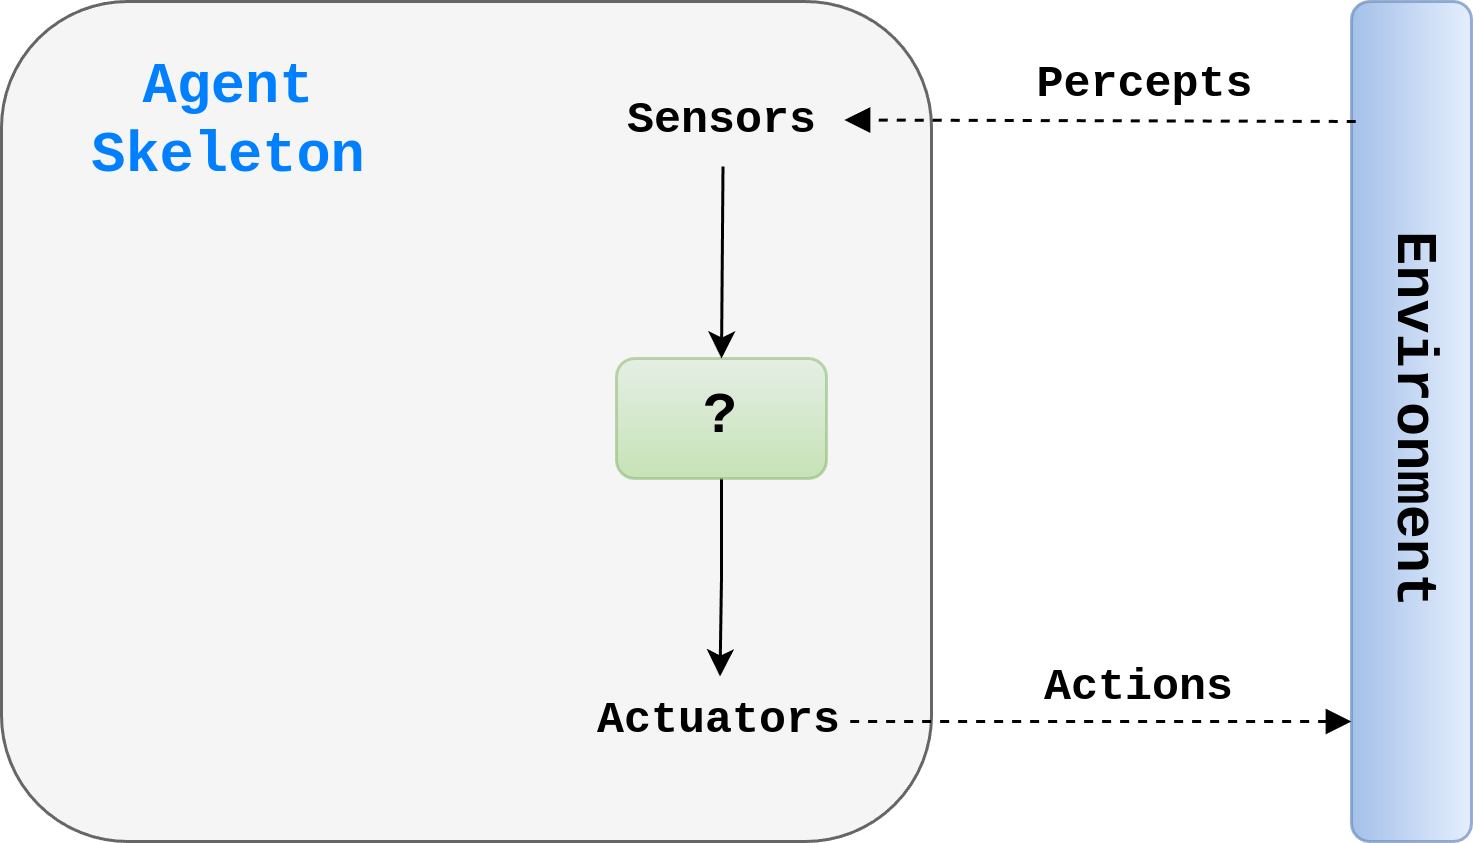
\includegraphics[
        width=0.5\linewidth,
        height=4cm,
        keepaspectratio
    ]{images/artificial-intelligence/ai-agents/agents-skeleton.png}
    \caption*{Agents interact with environments through sensors and actuators. \cite{common/online/tools/draw.io}}
\end{figure}


\begin{enumerate}
    \item \textbf{Agent}: An agent is anything that can be viewed as perceiving its environment through sensors and acting upon that environment through actuators.
    \hfill \cite{ai/book/Artificial-Intelligence-A-Modern-Approach/Russell-Norvig}
    \\
    \verb|agent = architecture + (agent) program|
    \hfill \cite{ai/book/Artificial-Intelligence-A-Modern-Approach/Russell-Norvig}

    \item \textbf{Environment}: environment refers to everything outside the agent that it interacts with.
    \hfill \cite{common/online/chatgpt}
    \\
    The “geography” of the environment is known \textbf{a priori}.
    \hfill \cite{ai/book/Artificial-Intelligence-A-Modern-Approach/Russell-Norvig}
    \\
    "A priori" : Knowledge or assumptions made before data is observed (e.g., predefined rules, constraints).
    \hfill \cite{common/online/chatgpt}

    \item \textbf{Sensors}: A sensor is any mechanism that allows an AI agent to perceive its environment by gathering information. This can be physical (hardware) or virtual (software).
    \hfill \cite{common/online/chatgpt}

    \item \textbf{Actuators}: An actuator is any mechanism that allows an AI agent to affect or change its environment by performing actions.
    \hfill \cite{common/online/chatgpt}

    \item \textbf{Percept}: agent’s perceptual inputs at any given instant
    \hfill \cite{ai/book/Artificial-Intelligence-A-Modern-Approach/Russell-Norvig}

    \item \textbf{Percept Sequence}: it is the complete history of everything the agent has ever perceived. In general, an agent’s choice of action at any given instant can depend on the entire percept sequence observed to date, but \textbf{not} on anything it hasn’t perceived.
    \hfill \cite{ai/book/Artificial-Intelligence-A-Modern-Approach/Russell-Norvig}

    \item \textbf{Agent Function}: maps any given percept sequence to an action; describes agent’s behavior; an external characterization of the agent; The agent function is an abstract mathematical description; takes the entire percept history
    \hfill \cite{ai/book/Artificial-Intelligence-A-Modern-Approach/Russell-Norvig}

    \item \textbf{Agent Program}: internal implementation of the agent function for an artificial agent; the agent program is a concrete implementation, running within some physical system. The agent program takes just the current percept as input because nothing more is available from the environment; if the agent’s actions need to depend on the entire percept sequence, the agent will have to remember the percepts.
    \hfill \cite{ai/book/Artificial-Intelligence-A-Modern-Approach/Russell-Norvig}

    \item \textbf{Architecture}: computing device with physical sensors and actuators on which the agent program is running.
    \hfill \cite{ai/book/Artificial-Intelligence-A-Modern-Approach/Russell-Norvig}

    \item \textbf{Performance Measure}: It evaluates any given sequence of environment states.
    \hfill \cite{ai/book/Artificial-Intelligence-A-Modern-Approach/Russell-Norvig}

    \item \textbf{Rational Agent}: A rational agent is one that does the right thing
    \hfill \cite{ai/book/Artificial-Intelligence-A-Modern-Approach/Russell-Norvig}
    \\
    For each possible percept sequence, a rational agent should select an action that is expected to maximize its performance measure, given the evidence provided by the percept sequence and whatever built-in knowledge the agent has.
    \hfill \cite{ai/book/Artificial-Intelligence-A-Modern-Approach/Russell-Norvig}
    \\
    Rationality is not the same as perfection.
    \hfill \cite{ai/book/Artificial-Intelligence-A-Modern-Approach/Russell-Norvig}
    \\
    Rationality maximizes \textbf{expected} performance, while perfection maximizes \textbf{actual} performance.
    \hfill \cite{ai/book/Artificial-Intelligence-A-Modern-Approach/Russell-Norvig}
    \\
    Our definition of rationality does not require omniscience, then, because the rational choice depends only on the percept sequence to date
    \hfill \cite{ai/book/Artificial-Intelligence-A-Modern-Approach/Russell-Norvig}


    \item \textbf{Omniscient Agent}: An omniscient agent knows the actual outcome of its actions and can act accordingly; but omniscience is impossible in reality.
    \hfill \cite{ai/book/Artificial-Intelligence-A-Modern-Approach/Russell-Norvig}


    \item \textbf{Information Gathering}: It is doing actions in order to modify future percepts.
    \hfill \cite{ai/book/Artificial-Intelligence-A-Modern-Approach/Russell-Norvig}



    \item When an agent is plunked down in an environment, it generates a sequence of actions according to the percepts it receives. This sequence of actions causes the environment to go through a sequence of states. If the sequence is desirable, then the agent has performed well.
    \hfill \cite{ai/book/Artificial-Intelligence-A-Modern-Approach/Russell-Norvig}

    \item  If we define success in terms of agent’s opinion of its own performance, an agent could achieve perfect rationality simply by deluding itself that its performance was perfect.
    \hfill \cite{ai/book/Artificial-Intelligence-A-Modern-Approach/Russell-Norvig}

    \item Human agents in particular are notorious for “sour grapes” - believing they did not really want something (e.g., a Nobel Prize) after not getting it.
    \hfill \cite{ai/book/Artificial-Intelligence-A-Modern-Approach/Russell-Norvig}

    \item As a general rule, it is better to design performance measures according to what one actually wants in the environment, rather than according to how one thinks the agent should behave.
    \hfill \cite{ai/book/Artificial-Intelligence-A-Modern-Approach/Russell-Norvig}

    \item The agent’s initial configuration could reflect some prior knowledge of the environment, but as the agent gains experience this may be modified and augmented. There are extreme cases in which the environment is completely known \textbf{a priori}. In such cases, the agent need not perceive or learn; it simply acts correctly. Such agents are fragile.
    \hfill \cite{ai/book/Artificial-Intelligence-A-Modern-Approach/Russell-Norvig}

    \item To the extent that an agent relies on the prior knowledge of its designer rather than on its own percepts, we say that the agent \textbf{lacks autonomy}.
    \hfill \cite{ai/book/Artificial-Intelligence-A-Modern-Approach/Russell-Norvig}
    \\
    A rational agent should be \textbf{autonomous} - it should learn what it can to compensate for partial or incorrect prior knowledge.
    \hfill \cite{ai/book/Artificial-Intelligence-A-Modern-Approach/Russell-Norvig}

    \item After sufficient experience of its environment, the behavior of a rational agent can become effectively \textbf{independent} of its prior knowledge. Hence, the incorporation of learning allows one to design a single rational agent that will succeed in a vast variety of environments.
    \hfill \cite{ai/book/Artificial-Intelligence-A-Modern-Approach/Russell-Norvig}


\end{enumerate}




\section{Task Environment/ Problem \cite{ai/book/Artificial-Intelligence-A-Modern-Approach/Russell-Norvig}}\label{AI: Agents/Task Environment or Problem}


\begin{enumerate}
    \item Task environments are essentially the “problems” to which rational agents are the “solutions.”
    \hfill \cite{ai/book/Artificial-Intelligence-A-Modern-Approach/Russell-Norvig}


\end{enumerate}

\subsection{PEAS: Defining Problem}

\begin{enumerate}
    \item \textbf{Performance}:
    \begin{enumerate}
        \item Desirable qualities
        \hfill \cite{ai/book/Artificial-Intelligence-A-Modern-Approach/Russell-Norvig}

        \item Defines how the success of the agent is evaluated.
        \hfill \cite{common/online/chatgpt}

        \item[] \textbf{Example}: In a self-driving car, performance can be measured by safety, fuel efficiency, and reaching the destination on time.
        \hfill \cite{common/online/chatgpt}
    \end{enumerate}

    \item \textbf{Environment}:
    \begin{enumerate}
        \item The surroundings in which the agent operates.
        \hfill \cite{common/online/chatgpt}

        \item[] \textbf{Example}: For a self-driving car, the environment includes roads, traffic, pedestrians, and weather conditions.
        \hfill \cite{common/online/chatgpt}
    \end{enumerate}

    \item \textbf{Actuators}:
    \begin{enumerate}
        \item The mechanisms that allow the agent to take action.
        \hfill \cite{common/online/chatgpt}

        \hfill Can be hardware or software.

        \item[] \textbf{Example}: A self-driving car uses its steering wheel, accelerator, and brakes as actuators.
        \hfill \cite{common/online/chatgpt}
    \end{enumerate}

    \item \textbf{Sensors}:
    \begin{enumerate}
        \item The components that allow the agent to perceive its environment.
        \hfill \cite{common/online/chatgpt}

        \hfill Can be hardware or software.

        \item[] \textbf{Example}: A self-driving car has cameras, LiDAR, GPS, and speed sensors.
        \hfill \cite{common/online/chatgpt}
    \end{enumerate}

\end{enumerate}


\vspace{0.3cm}

\textbf{Note}:
\begin{enumerate}
    \item some \textbf{software agents} (or \textbf{software robots} or \textbf{softbots}) exist in rich, unlimited domains.
    \hfill \cite{ai/book/Artificial-Intelligence-A-Modern-Approach/Russell-Norvig}


\end{enumerate}


\clearpage
\subsection{Properties of Task Environments \cite{ai/book/Artificial-Intelligence-A-Modern-Approach/Russell-Norvig}}

\subsubsection{Fully observable, partially observable, unobservable}
\begin{enumerate}
    \item \textbf{fully observable}: If an agent’s sensors give it access to the complete state of the environment at each point in time, then we say that the task environment is fully observable.
    A task environment is effectively fully observable if the sensors detect all aspects that are \textbf{relevant} to the choice of action; relevance, in turn, depends on the performance measure.
    Fully observable environments are convenient because the agent need not maintain any internal state to keep track of the world.
    \hfill \cite{ai/book/Artificial-Intelligence-A-Modern-Approach/Russell-Norvig}

    \vspace{0.2cm}

    \item \textbf{partially observable}: An environment might be partially observable because of noisy and inaccurate sensors or because parts of the state are simply missing from the sensor data.
    \hfill \cite{ai/book/Artificial-Intelligence-A-Modern-Approach/Russell-Norvig}

    \vspace{0.2cm}

    \item \textbf{unobservable}: If the agent has no sensors at all then the environment is unobservable.
    The agent’s goals may still be achievable, sometimes with certainty.
    \hfill \cite{ai/book/Artificial-Intelligence-A-Modern-Approach/Russell-Norvig}
\end{enumerate}

\subsubsection{Single agent, multi-agent}
\begin{enumerate}
    \item \textbf{Single agent}:  Only 1 agent is interacting in the given environment.

    \item \textbf{Multi-agent}: More than 1 agent (of same type or different types) interact in the given environment.
    \begin{enumerate}
        \item \textbf{Competitive Multi-agent}: Agents maximize their own performance at cost of other agents' performance.
        \\
        Examples: 2 agents playing Chess against each other; taxi-driving (competing for parking space)

        \item \textbf{Cooperative Multi-agent}: Agents take actions to maximize collective performance.
        \\
        Example: taxi-driving (avoiding collisions)

        \vspace{0.3cm}

        \item \textbf{communication} often emerges as a rational behavior in multiagent environments; in some competitive environments, \textbf{randomized behavior} is rational because it avoids the pitfalls of predictability.
        \hfill \cite{ai/book/Artificial-Intelligence-A-Modern-Approach/Russell-Norvig}
    \end{enumerate}

\end{enumerate}


\subsubsection{Deterministic, stochastic, uncertain, nondeterministic}
\begin{enumerate}
    \item If the next state of the environment is completely determined by the current state and the action executed by the agent, then we say the environment is \textbf{deterministic}; otherwise, it is \textbf{stochastic}.
    \hfill \cite{ai/book/Artificial-Intelligence-A-Modern-Approach/Russell-Norvig}

    \item In principle, an agent need not worry about uncertainty in a fully observable, deterministic environment.
    \hfill \cite{ai/book/Artificial-Intelligence-A-Modern-Approach/Russell-Norvig}

    \item  If the environment is partially observable, however, then it could appear to be stochastic. Most real situations are so complex that it is impossible to keep track of all the unobserved aspects; for practical purposes, they must be treated as \textbf{stochastic}.
    \hfill \cite{ai/book/Artificial-Intelligence-A-Modern-Approach/Russell-Norvig}
    \\
    It implies that uncertainty about outcomes is quantified in terms of \textit{probabilities}.
    \hfill \cite{ai/book/Artificial-Intelligence-A-Modern-Approach/Russell-Norvig}

    \item  We say an environment is \textbf{uncertain} if it is not fully observable or not deterministic.
    \hfill \cite{ai/book/Artificial-Intelligence-A-Modern-Approach/Russell-Norvig}

    \item A \textbf{nondeterministic} environment is one in which actions are characterized by their possible outcomes, but no probabilities are attached to them. Non-deterministic environment descriptions are usually associated with performance measures that require the agent to succeed for all possible outcomes of its actions.
    \hfill \cite{ai/book/Artificial-Intelligence-A-Modern-Approach/Russell-Norvig}
\end{enumerate}


\subsubsection{Episodic, sequential}
\begin{enumerate}
    \item In an \textbf{episodic} task environment, the agent’s experience is divided into atomic episodes. In each episode the agent receives a percept and then performs a single action. Crucially, the next episode does not depend on the actions taken in previous episodes. Episodic environments are much simpler than sequential environments because the agent does not need to think ahead.
    \hfill \cite{ai/book/Artificial-Intelligence-A-Modern-Approach/Russell-Norvig}

    \item In \textbf{sequential} environments, on the other hand, the current decision could affect all future decisions.
    \hfill \cite{ai/book/Artificial-Intelligence-A-Modern-Approach/Russell-Norvig}
\end{enumerate}


\subsubsection{Static, dynamic, semidynamic}
\begin{enumerate}
    \item If the environment can change while an agent is deliberating, then we say the environment is \textbf{dynamic} for that agent; otherwise, it is \textbf{static}.
    \hfill \cite{ai/book/Artificial-Intelligence-A-Modern-Approach/Russell-Norvig}

    \item Static environments are easy to deal with because the agent need not keep looking at the world while it is deciding on an action, nor need it worry about the passage of time.
    \hfill \cite{ai/book/Artificial-Intelligence-A-Modern-Approach/Russell-Norvig}

    \item  Dynamic environments, on the other hand, are continuously asking the agent what it wants to do; if it hasn’t decided yet, that counts as deciding to do nothing.
    \hfill \cite{ai/book/Artificial-Intelligence-A-Modern-Approach/Russell-Norvig}

    \item If the environment itself does not change with the passage of time but the agent’s performance score does, then we say the environment is \textbf{semidynamic}.
    \hfill \cite{ai/book/Artificial-Intelligence-A-Modern-Approach/Russell-Norvig}
\end{enumerate}


\subsubsection{Discrete, continuous}
\begin{enumerate}
    \item The discrete/continuous distinction applies to the state of the environment, to the way \textit{time} is handled, and to the percepts and actions of the agent.
    \hfill \cite{ai/book/Artificial-Intelligence-A-Modern-Approach/Russell-Norvig}


\end{enumerate}



\subsubsection{Known, unknown}
\begin{enumerate}
    \item Strictly speaking, this distinction refers not to the environment itself but to the agent’s (or designer’s) state of knowledge about the “laws of physics” of the environment.
    \hfill \cite{ai/book/Artificial-Intelligence-A-Modern-Approach/Russell-Norvig}

    \item In a \textbf{known} environment, the outcomes (or outcome probabilities if the environment is stochastic) for all actions are given.
    \hfill \cite{ai/book/Artificial-Intelligence-A-Modern-Approach/Russell-Norvig}

    \item  if the environment is \textbf{unknown}, the agent will have to learn how it works in order to make good decisions.
    \hfill \cite{ai/book/Artificial-Intelligence-A-Modern-Approach/Russell-Norvig}


\end{enumerate}



\subsubsection*{Examples \cite{ai/book/Artificial-Intelligence-A-Modern-Approach/Russell-Norvig}}

\begin{customArrayStretch}{1.3}
\begin{tabular}{ | >{\fontsize{10}{10}\arraybackslash}l | l l l l l l | }
    \hline

    \textbf{Task Environment} & \textbf{Observable} & \textbf{Agents} &
        \textbf{Deterministic} & \textbf{Episodic} &
        \textbf{Static} & \textbf{Discrete} \\

    \hline\hline

    \textbf{Crossword puzzle} & Fully & Single & Deterministic & Sequential & Static & Discrete \\

    \textbf{Chess with a clock} & Fully & Multi & Deterministic & Sequential & Semi & Discrete \\

    \hline

    \textbf{Poker} & Partially & Multi & Stochastic & Sequential & Static & Discrete \\

    \textbf{Backgammon} & Fully & Multi & Stochastic & Sequential & Static & Discrete \\

    \hline

    \textbf{Taxi driving} & Partially & Multi & Stochastic & Sequential & Dynamic & Continuous \\

    \textbf{Medical diagnosis} & Partially & Single & Stochastic & Sequential & Dynamic & Continuous \\

    \hline

    \textbf{Image analysis} & Fully & Single & Deterministic & Episodic & Semi & Continuous \\

    \textbf{Part-picking robot} & Partially & Single & Stochastic & Episodic & Dynamic & Continuous \\

    \hline

    \textbf{Refinery controller} & Partially & Single & Stochastic & Sequential & Dynamic & Continuous \\

    \textbf{Interactive English tutor} & Partially & Multi & Stochastic & Sequential & Dynamic & Discrete \\

    \hline
\end{tabular}
\end{customArrayStretch}



\subsubsection*{Note}
\begin{enumerate}
    \item  the distinction between known and unknown environments is not the same as the one between fully and partially observable environments.
    \hfill \cite{ai/book/Artificial-Intelligence-A-Modern-Approach/Russell-Norvig}

    \item It is quite possible for a \textbf{known} environment to be \textbf{partially observable}—for example, in solitaire card games, I know the rules but am still unable to see the cards that have not yet been turned over.
    \hfill \cite{ai/book/Artificial-Intelligence-A-Modern-Approach/Russell-Norvig}

    \item an \textbf{unknown} environment can be \textbf{fully observable}—in a new video game, the screen may show the entire game state but I still don’t know what the buttons do until I try them.
    \hfill \cite{ai/book/Artificial-Intelligence-A-Modern-Approach/Russell-Norvig}

    \item \textbf{environment class}: A category or set of related environments from which specific environments are drawn for testing or training agents.
    \hfill \cite{ai/book/Artificial-Intelligence-A-Modern-Approach/Russell-Norvig, common/online/chatgpt}

    \item \textbf{environment generator}: An environment generator is a tool or function that creates individual environments sampled from an environment class. It automates the creation of diverse scenarios for training or evaluating agents.
    \hfill \cite{ai/book/Artificial-Intelligence-A-Modern-Approach/Russell-Norvig, common/online/chatgpt}


\end{enumerate}



\section{Agent State Representations}\label{AI: Agents/Agent State Representations}

\begin{figure}[H]
    \centering
    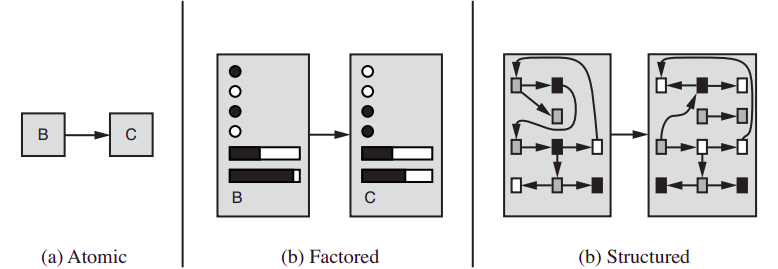
\includegraphics[
        width=\linewidth,
        height=6cm,
        keepaspectratio,
    ]{images/artificial-intelligence/ai-agents/state-representations.png}
    \caption*{
    Three ways to represent states and the transitions between them.
    \\
    \textbf{(a)} Atomic representation: a state (such as B or C) is a black box with no internal structure;  
    \hfill \cite{ai/book/Artificial-Intelligence-A-Modern-Approach/Russell-Norvig}
    \\
    \textbf{(b)} Factored representation: a state consists of a vector of attribute values; values can be Boolean, realvalued, or one of a fixed set of symbols.
    \hfill \cite{ai/book/Artificial-Intelligence-A-Modern-Approach/Russell-Norvig}
    \\
    \textbf{(c)} Structured representation: a state includes objects, each of which may have attributes of its own as well as relationships to other objects.
    \hfill \cite{ai/book/Artificial-Intelligence-A-Modern-Approach/Russell-Norvig}
}
\end{figure}



\begin{enumerate}[itemsep=0.2cm]
    \item Roughly speaking, a more expressive representation can capture, at least as concisely, everything a less expressive one can capture, plus some more. 
    \hfill \cite{ai/book/Artificial-Intelligence-A-Modern-Approach/Russell-Norvig}

    \item Often, the more expressive language is much more concise; for example, the rules of chess can be written in a page or two of a structured-representation language such as first-order logic but require thousands of pages when written in a factored-representation language such as propositional logic.
    \hfill \cite{ai/book/Artificial-Intelligence-A-Modern-Approach/Russell-Norvig}

    \item reasoning and learning become more complex as the expressive power of the representation increases.
    \hfill \cite{ai/book/Artificial-Intelligence-A-Modern-Approach/Russell-Norvig}

    \item To gain the benefits of expressive representations while avoiding their drawbacks, intelligent systems for the real world may need to operate at all points along the axis simultaneously.
    \hfill \cite{ai/book/Artificial-Intelligence-A-Modern-Approach/Russell-Norvig}
\end{enumerate}






\subsection{Atomic representation}

\begin{enumerate}[itemsep=0.2cm]
    \item each state of the world is indivisible - it has no internal structure. 
    \hfill \cite{ai/book/Artificial-Intelligence-A-Modern-Approach/Russell-Norvig}

    \item two different atomic states have nothing in common—they are just different black boxes
    \hfill \cite{ai/book/Artificial-Intelligence-A-Modern-Approach/Russell-Norvig}

    \item Algorithms/ areas that work with atomic representations - or, at least, they treat representations as if they were atomic:
    \begin{enumerate}
        \item Search and game-playing
        \hfill \cite{ai/book/Artificial-Intelligence-A-Modern-Approach/Russell-Norvig}

        \item Hidden Markov models
        \hfill \cite{ai/book/Artificial-Intelligence-A-Modern-Approach/Russell-Norvig}

        \item Markov decision processes
        \hfill \cite{ai/book/Artificial-Intelligence-A-Modern-Approach/Russell-Norvig}
    \end{enumerate}
\end{enumerate}



\subsection{Factored representation}

\begin{enumerate}[itemsep=0.2cm]
    \item A factored representation splits up each state into a fixed set of \textbf{variables} or \textbf{attributes}, each of which can have a \textbf{value}.
    \hfill \cite{ai/book/Artificial-Intelligence-A-Modern-Approach/Russell-Norvig}

    \item two different factored states can \textbf{share} some attributes (such as being at some particular GPS location) and not others (such as having lots of gas or having no gas)
    \\
    this makes it much easier to work out how to turn one state into another
    \hfill \cite{ai/book/Artificial-Intelligence-A-Modern-Approach/Russell-Norvig}

    \item With factored representations, we can also represent uncertainty - for example, ignorance about the amount of gas in the tank can be represented by leaving that attribute blank.
    \hfill \cite{ai/book/Artificial-Intelligence-A-Modern-Approach/Russell-Norvig}

    \item Algorithms/ areas based on factored representations:
    \begin{enumerate}
        \item constraint satisfaction algorithms
        \hfill \cite{ai/book/Artificial-Intelligence-A-Modern-Approach/Russell-Norvig}

        \item propositional logic
        \hfill \cite{ai/book/Artificial-Intelligence-A-Modern-Approach/Russell-Norvig}

        \item planning
        \hfill \cite{ai/book/Artificial-Intelligence-A-Modern-Approach/Russell-Norvig}

        \item Bayesian networks
        \hfill \cite{ai/book/Artificial-Intelligence-A-Modern-Approach/Russell-Norvig}

    \end{enumerate}
\end{enumerate}








\subsection{Structured representation}


\begin{enumerate}[itemsep=0.2cm]
    \item the world as having things in it that are related to each other, not just variables with values.
    \hfill \cite{ai/book/Artificial-Intelligence-A-Modern-Approach/Russell-Norvig}

    \item almost everything that humans express in natural language concerns objects and their relationships
    \hfill \cite{ai/book/Artificial-Intelligence-A-Modern-Approach/Russell-Norvig}

    \item Algorithms/ areas based on factored representations:
    \begin{enumerate}
        \item relational databases
        \hfill \cite{ai/book/Artificial-Intelligence-A-Modern-Approach/Russell-Norvig}

        \item first-order logic
        \hfill \cite{ai/book/Artificial-Intelligence-A-Modern-Approach/Russell-Norvig}

        \item first-order probability models 
        \hfill \cite{ai/book/Artificial-Intelligence-A-Modern-Approach/Russell-Norvig}

        \item knowledge-based learning
        \hfill \cite{ai/book/Artificial-Intelligence-A-Modern-Approach/Russell-Norvig}

        \item natural language understanding
        \hfill \cite{ai/book/Artificial-Intelligence-A-Modern-Approach/Russell-Norvig}
    \end{enumerate}
\end{enumerate}





